\documentclass[11pt]{article}
\usepackage{todonotes}
\usepackage{float}
\usepackage[backend=biber,style=authoryear,maxcitenames=2,url=false]{biblatex}
%\bibliography{bibevol2.bib}
\bibliography{bibevol.bib}
%\bibliography{bibevol3.bib}
\bibliography{bibevol4.bib}
\usepackage{sgame}
\usepackage{tikz}
\usepackage{pgfplots}
 % Useful for Physics related math
\usepackage{physics}
\usepackage{amsmath}
\usepackage{amssymb} 
\usepackage{amsthm}
        % packages that allow mathematical formatting
\usepackage{setspace}
\setlength\parindent{0pt}
        % set space and indent and indent
\usepackage{hyperref}
\hypersetup{
            colorlinks,
                linkcolor={red!50!black},
                    citecolor={blue!50!black},
                        urlcolor={blue!80!black}
                }
\usepackage[a4paper,width=150mm,top=25mm,bottom=25mm]{geometry}

% New commands
\let\conju\overline
\newcommand\numberthis{\addtocounter{equation}{1}\tag{\theequation}}
\newcount\colveccount
\newcommand*\colvec[1]{
        \global\colveccount#1
        \begin{pmatrix}
                \colvecnext
        }
        \def\colvecnext#1{
                #1
                \global\advance\colveccount-1
                \ifnum\colveccount>0
                \\
                \expandafter\colvecnext
                \else
        \end{pmatrix}
        \fi
}
        % Columnvectors
\newtheorem{mydef}{Definition}

\pgfplotsset{compat=1.11}
\linespread{1.5}
\newcommand{\natnumb}{\mathbb{N}}
\newcommand{\realnumb}{\mathbb{R}}
\presetkeys{todonotes}{color=yellow,size=\scriptsize}{}
\begin{document}
\section{Introduction}
\begin{figure}[h]
\begin{center}
\begin{game}{2}{2} & $S$ & $H$
\\ $S$ &$a,a$ &$b,c$
\\ $H$ &$c,b$ &$d,d$ \end{game}
\label{sh}
\end{center}
\caption{A parametrized form of the Stag hunt game, $a>c\geq d >b$}
\end{figure}
\section{The Stag hunt game}
\label{sec:traditional}
\todo{Motivation of traditional game theory}
As introduced, the stag hunt game is played by two players who choose their
strategies simultaneoulsy. Both have information about the strategies of the
other player and the payoffs they and their opponents receive. In game theory
such a game is called a \textit{normalform} game. Typically, such a game is
formalized as a Triplet $\Gamma = (I,\mathbb{S},F)$, with the set of players 
$I=\{1,2,...,n\}$, where $n$ is the total number of players, 
the pure strategy space of the game $S = \times_i S_i$
with the pure strategy space $S_i$ of an individual player 
$i \in I$ defined as $S_i = \{1,2,...,m_i\}$, where $m_i$ denotes the total
number of strategies available to player $i$, and the payoff function 
$F: S \rightarrow \realnumb^n$.
As this text focusses on the stag hunt game, which is a normalform game,
this definitons reduce to the following.
By setting $n=2$, we define the two hunters playing SH as $I=\{1,2\}$. A 
player $i \in I$  can choose from a set of pure strategies from his 
pure strategy space, $S_i$. Those strategies are called pure, because they 
differ from the later defined mixed strategies. In the SH game, 
each hunter can choose out of two pure strategies, namely, huntig the stag 
(strategy 1) or hunting hare (strategy 2).
Therefore, the pure strategy space is defined by $S_i = {1,2}$, which results
from definiton ???? by setting $m_i$. In the SH game both players choose from
the same set of stragies such that $S_1 =S_1=S$. Combining the strategy spaces
of the two players with the cartesian product
yields the definiton of the pure strategy space of the game
$\mathbb{S}= S \times S = S^2$.

In SH the hunters do not just hunt for their pleasure \todo{Hunter bewerten 
Ausgang des Spiels}\footnote{Even though the
situation would not differ, aslong as we assume the pleasure hunting a stag
to be higher than hunting hare, since economically payoffs are interpreted as
utility in the theory of households.}, but to seek 
a reward for their loot. This is captured by the definition of an individual
payoff function $F_i:S \rightarrow \realnumb$, which maps for a player $i \in
I$ to every state of the game $s=(s_1,s_2) \in S^2$, where $s_i$ is a 
pure strategy of player $i$, a payoff $F_i(s) \in \realnumb$. So
every outcome of the game, every combination of strategies the players could
individually choose, is defined. In the special case of two player, one 
can define a payoff matrix for player 1 $A \in \realnumb^{2 \times2}$ and for 
player 2  $B \in \realnumb^{2 \times2}$, where $A_{kl} = F_1(k,l)$ and $
B_{kl} = F_2(k,l)$ with the pure strategies $k,l \in S$. Using the 
representation above, one can indentify the payoff matrices for the player as
\begin{align}
        A = \mqty(a && b \\ c && d), \quad B = \mqty(a && c \\ b && d)
        \label{eq:matrix}
\end{align}

In the study of games, one is interested in defining subclasses of games.
For the game here in study the following definition is important: 
\begin{mydef}
        A two player game $\Gamma=(I,S_1 \times S_2, A,B)$ is called symmetric
        if the players of the game have the same strategy space $S_1=S_2=S$ and
        for the payoff matrices the condition $B=A^T$ holds. Therefore, the
        game is well-defined as $\Gamma=(I,S^2,A)$.
        \label{symmetry}
\end{mydef}
Clearly, the SH game is such a game. Both hunters have the same strategies 
available and the payoff matrices defined in \todo{Richtiges Nummerieren der 
Gleichungen} \eqref{eq:matrix} fulfill the required condition in Definition
\ref{symmetry}. Hence, it is irrelevant which player we label 1 or 2.


Usually a game is extended by the possibility of the players to play
\textit{mixed strategies}. Intuitively, in the analogy of SH, one can think of
such strategies as that a hunter decides whether to shoot the stag or the hare
by flipping a coin which shows head or tails, not necessarily with an equal
probabillity.\todo{Interpretation intuitively problematic e.t.c.} Formally, every player of the game assigns a probabillity 
distribution over his pure strategies space.  
A strategy $x_i \in \Delta_i$ of player $i \in I$ 
is called a \textit{mixed strategy}, where $\Delta_i$ is the mixed strategy 
space 
\begin{align*}
        \Delta_i = \{ x_i \in \realnumb^2 : \sum_{k \in S} x_{ik} = 1, x_{ik} \geq 0 \quad
\forall k \in S\}.
\end{align*}
Since there is no restriction for any players choice of the probabillity 
distribution, in a symmetric game the mixed strategy spaces of the players
also equal. For the SH game this means $\Delta_1 = \Delta_2 = \Delta$.
With this notation a pure strategy can be interpreted as a mixed strategy
which assigns probabillity one to the pure strategy chosen and zero to all
other strategies. This is represented by the unit vectors of the simplex 
$\hat{e}_k \in \Delta$, $\hat{e}_1 = (1,0)^T$ is the pure strategy hunting stag 
and $\hat{e}_2 =(0,1)^T$ denots the pure strategy hunting hare.
Similiar to the pure strategy case, the mixed strategy spaces of the players 
$\Delta$ is combined to the mixed strategy space of the game $\Delta^2 =
\Delta \times \Delta$. From now on $x \in \Delta$ denotes a (mixed) strategy
chosen by player 1 and $y \in \Delta$ a (mixed) strategy of player 2.
Again similiar to the pure strategy case, the mixed strategy payoff 
$\hat{F}_i:\Delta^2 \rightarrow \realnumb$ maps to any state in the mixed strategy
space  $(x,y) \in \Delta^2$ a payoff $\hat{F}_i(x,y) \in \realnumb$.
With the matrix notation this is defined as: 
\begin{alignat*}{2}
        \hat{F}_1(x,y) &= x^T A y \\
        \hat{F}_2(x,y) &= x^T A^T y 
\end{alignat*}

Finally, the SH game is formally defined as a symmetric two-player normal form
game $\Gamma = (I=\{1,2\}, \Delta^2, \hat{F})$.

\subsection{Traditional concepts}
In describing the behavior of agents game theory developed a wide range of 
tools to solve this strategic interactions. \todo{Rationality assumption and
Equilibrium knowledge required for Nash equilibrium}

The \textit{best-reply} for player $i \in I$ to a strategy $y \in \Delta$ 
played by $j \neq i$ is defined as:
\begin{align}
        \beta(y) = \{x \in \Delta: \hat{F}(x,y) \geq \hat{F}(x',y), 
        \quad \forall x' \in \Delta\}
\end{align}
This formally assigns to each strategy of the other player the strategies
of player $i$ resulting in the highest payoff for player $i$. However, a player
must be capable of computing his best-reply to a given strategy.

The most famous and used traditional solution concept, the \textit{Nash 
equilibrium} assumes this kind of capability of each individual players. 
The Nash equilibrium was named by its proposer J. Nash in 1950 
just referred to as equilibrium.

A Nash equilibrium for the SH game is defined as
\begin{mydef}
        \label{def:nashequilibrium}
        A state of $(x^*,y^*) \in \Delta^2$ is called a Nash equilibrium if 
        it holds that\todo{Nicer form}
\begin{itemize}
        \item   $(x^*)^T A y^* \geq x^T A y^*, \quad \forall x \in \Delta$
        \item   $(x^*)^T A y^* \geq (x^*)^T A y, \quad \forall y \in \Delta$.
\end{itemize}
It is called symmetric if $x^* = y^*$. A Nash equilibrium is 
strict Nash equilibrium if the inequality is strict.
\end{mydef}
Equivalently, both players choose a best-reply in the Nash equilibrium.
One can proof that in every normal form game with mixed 
strategies a Nash equilibrium exists. This existence proof is due to 
\textcite{nash_equilibrium_1950}.

The SH game admits three symmetric Nash equilibria. The first one consists
of both players choosing strategy 1, hunting stag, $(\hat{e}_1,\hat{e}_1) \in
\Delta^2$, where both players receive the payoff $a$. 
None of both has an incentive to change his decision. For both
playing the pure strategy 1 is a best-reply because a unilateral deviation 
leads to the payoff $c \leq a$.
The second equilibrium is the state of 
both players choosing strategy 2, hunting hare, $(\hat{e}_2,\hat{e}_2)
\in \Delta^2$. Again by definition, both play a best-reply and a unilateral 
deviation of a player results in a lower payoff $b<d$.
Additionally to this Nash equilibria in pure strategies, there is a symmetric
mixed-strategy equilbrium assigning a probability $q=\frac{d-b}{a-c+d-b}$ to
strategy 1. To see this, calculating the pay \todo{Calculation that payoff is
not dependend what strategy is chosen againt q}

For further analysis it is convenient to use that Nash equilibria are only
defined by a difference inequality. Hence, any affine transformation of the
payoff matrix and \textit{local shifts} do not change the set of Nash equilibria 
of the game \parencite[17-19]{weibull_evolutionary_1997}. A transformation is
called a local shift if to all payoffs in a column of the payoff matrix for 
a player the same constant is added. Formally, let $A_{ij}$ denote the 
elements of the player's payoff matrix, a local shift to column $j^*$ 
transform this payoff
matrix into the payoff matrix $A^*$ as:
\begin{align}
        A^*_{ij} =
        \begin{cases}
                A_{ij} + v & \text{for}\ j=j^*, v \in \realnumb \\
                A_{ij}
        \end{cases}
\end{align}
This does not change the best-reply structures of the normal form game,
since it does not the change the differences a player considers when valuating
which strategy is better against a given strategy of the other player. When 
applying this to the stag hunt game one can use two local shifts to get
the shifted payoff matrix with the diagonal elements $A_{11}=\alpha_1$ and 
$A_{22}=\alpha_2$, where $\alpha_1=a-c$ and $\alpha_2=d-b$ and 
zero off the diagonal. \textcite[28]{weibull_evolutionary_1997} 
groups all symmetric 2x2 games into four categories with different 
equilibrium properties. Outlined in the discussion, the stag hunt game 
is considered as a coordination game, with $\alpha_1, \alpha_2 > 0$
and in contrast to the three other categories the solution is not so obvious.
I will discuss this in the section concerning the selection of an equilibria 
\ref{sec:equilibriumselection}.

\subsection{Evolutionary concepts}
The stag hunt game has multiple Nash equilibria. But which equilibrium will
no be played one might ask. Answering this question, game theorists tried
to construct refinements of the Nash equilibria in cases where some Nash
equilibria seemed to be unconvincing. Motivated by the context of evolution
in animal populations \cite{maynard} constructed the refinement 
\textit{Evolutionary stable strategy} (ESS). In his model, animals are of a
specific phenotype, representing strategies, playing a normal form game where
the payoffs are not directly measured in utility but represent the darwinian 
fitness of that phenotyp, i.e. the expected number of offsprings to that
phenotype. A crucial difference to the games traditional game theory considers, 
played by agents with a fair amount of ability to calculate best-replies,
is that the animals \textit{are} of a phenotyp and cannot change it by will.
They cannot \textit{choose} their "strategy" in the game like agents do.
Biologists then ask which composition of the population cannot be invaded.
Formally, this intuition leads for a symmetric
two-player game to
\begin{mydef}
        \label{def:ess}
        A strategy $x \in \Delta$ is called evolutionary stable (ESS) if it
        holds that
        \begin{align*}
                \label{eq:essinvasion}
                \hat{F}(x,\epsilon y + (1-\epsilon) x) > 
                \hat{F}(y,\epsilon y + (1-\epsilon) y), \numberthis
        \end{align*}
        where $y \in \Delta, y \neq x$ is the strategy of the group invading the
        existing population with share $\epsilon \in (0,1)$.
        Alternatively, the ESS $x$ satisfies
        \begin{alignat}{2}
                \label{eq:essstrict}
                \hat{F}(x,x) &\geq \hat{F}(y,x) \forall y \\ 
                \hat{F}(y,x) &= \hat{F}(x,x) \Rightarrow  
                \hat{F}(y,y) < \hat{F}(x,y) \label{eq:essstrict2}
        \end{alignat}
\end{mydef}
The first part of the definition depicts the intution of an invasion in the
population context.
Hence, the highest share $\bar{\epsilon}$ of $y$ the evolutionary stable 
strategy $x$  can be invaded such that the inequality in definition 
\ref{def:ess} holds for any $\epsilon \in (0,\bar{\epsilon})$ is called  
\textit{invasion barrier} \cite{weibull_evolutionary_1997}. 
The alternative defintion in \eqref{eq:essstrict} and \eqref{eq:essstrict2}
shows why it is called an refinement of the Nash equilibrium. Indeed,
seen in \eqref{eq:essstrict}, an ESS is used in a Nash equilibrium as it 
needs to be a best-reply to satisfy the ESS condition. In addition, 
a strategy used in a strict Nash equilibrium is always an ESS, 
since it directly satisfies 
\eqref{eq:essstrict}. The equivalence of both formulations is shown in
\cite{weibull_evolutionary_1997}.
Not all strategies in the equilibria of the stag hunt game are evolutionary
stable strategies. The pure strategies $e_1$ and $e_2$ are evolutionary stable,
since both symmetric equilibria consisting of them are strict and so 
satisfy the condition \eqref{eq:essstrict}. The strategy assigning 
a probability of $q=\frac{\alpha_1}{\alpha_1 + \alpha_2}$ used in the 
mixed equilibrium is not an ESS, because condition \eqref{eq:essstrict} is
an equality and the implication of \eqref{eq:essstrict2} does not hold for all
strategies $y \in \Delta$.
Consider for example $y =(e_1,e_1)$ the pure strategy $e_1$. It follows that
$\hat{F}((q,1-q),y) = \frac{\alpha_1 \alpha_2}{\alpha_1+\alpha_2}
< \alpha_1 = \hat{F}(y,y)$, violating inequality \eqref{eq:essstrict2}.

In section \ref{sec:replciatordynamic}, the connection of the ESS refinement
and evolutionary dynamics will become clearer. Especially the first formulation
of an ESS in equation \eqref{eq:ess} will be justified.

\subsection{Equilibrium Selection}
\label{sec:equilibriumselection}
Clearly, game theory has the aspiration to provide advise for agents in 
situations such as that defined above.
As seen in the stag hunt game, the mostly used solution concept, 
the Nash equilibrium, and refinements such as the ESS are
not sufficient to select a unique equilibrium, even in the case of a simple
2x2 game. This does not satisfy game theorists since it is not clear which
equilibrium is finally played by the agents. Or how \cite{weibull} puts it,
this kind of coordination games "caused\footnote{And still causes} game theorists and users of 
noncooperative game theory a fair amount of frustration". 

A closer look at the two pure Nash equilibria in the Stag hunt game 
shows their differences. Considering the normal form representation in figure 
\ref{sh}, the Nash equilibrium where both players choose strategy one has the highest payoff
for both players. It is then said that $(\hat{e}_1,\hat{e}_2)$ 
\textit{Pareto-dominates} $(\hat{e}_2,\hat{e}_2)$. In the other standard 
normal form game describing a social-dilemmata, the Prisoners Dilemma, as 
shown in figure \ref{pd} the Pareto-dominant outcome is not a 
Nash equilibrium\footnote{This is true for one-shot games. 
In repeated games there is the possibility in ending at the Pareto efficient 
outcome.}, because every agent has the incentive to deviate. In the stag hunt
game this is not the case. Every agent plays a best-reply in the Pareto efficient
outcome, but since there is another Nash equilibrium it is not clear 
which one is played based on this criterion alone. Based on \cite{schelling}
one may argue that Pareto-dominance characterizes $(\hat{e}_1,\hat{e}_1)$ 
as a focal point of the game, a solution of the game which makes the most sense
to play but the reasons for this are abstracted away from the strategic form and are consens among
the players. \todo{Focal points definition} However, the equilibrium point
$(\hat{e}_2,\hat{e}_2)$ exhibits the feature of \textit{Risk-Dominance}. 
\cite{seltenharsanyigeneral} defined this selection criterion based on the
risk for the players associated with an equilibrium point. Formally, in the
SH game, 
\begin{mydef}
The Nash equilibrium $x=(\hat{e}_2,\hat{e}_2)$ \textit{risk-dominates} 
         the Nash equilibrium $y=(\hat{e}_1,\hat{e}_1)$, if $d-b > a-c$.
         \label{riskdom}
 \end{mydef}\todo{Maybe change this definition}
 As mentioned in \cite{weibull_evolutionary_1997} a NE risk-dominates, if it is Pareto-efficient
 in the reduced payoff version of the game, associated with the diagonal
 payoff matrix in \eqref{diagmatrix}, as the definition \ref{riskdom} 
 corresponds to $\alpha_1 < \alpha_2$.
So both pure Nash equilibria have a certain appeal for game theorists to be
favored. Indeed, there is no clear consent which equilibrium will be played. 
\cite{aumann} argues that communication before the game would lead to 
an agreement on the Pareto-dominant equilibrium.\todo{Cheap talk: Find the paper
Aumann 1990}
Although Harsanyi and Selten introduced the Risk-dominance criterion in 
\cite{seltenharsanyigeneral}, their general theory favors Payoff-dominance in the
Stag hunt case. On the hand, Harsanyi, as Aumann, later advocates in \cite{harsanyinew} 
for the Risk-dominant criterion. 

The evolutionary approach outlined in the next section may contribute to 
the equilibrium selection problem. 

\section{The Evolutionary Game}
\label{evolutionarysection}
Evolutionary game theory, started by Maynard Smith, has find a lot of 
recognition in the game theory literature. \todo{Applications and stuff}

In an evolutionary game, a population of agents interacts in a 
strategic environment. It is usually assumed that the number of agents is 
large, such that an individual agents decision has a small effect on the
state of the population. This is called a \textit{population game} \cite{sandholm_population_2010}.

An evolutionary stag hunt game then consists of agents in a population who
are randomly matched against each other playing the normal form game 
$\Gamma = (I,\Delta^2,\hat{F})$ discussed before. In a \textit{monomorphic}\footnote{In 
contrast to \textit{polymorhpic} populations where each agent can also 
play mixed strategies} setting, the agents are only able to play pure 
strategies. As both settings do not differ in their main implications, 
monomorphic populations admit a handy interpretation for mixed-strategies\todo{Citation, What is Game Theory Trying to accomplish}.
Let $p_j(t) \geq 0$ be the number of individuals playing strategy $j \in \{1,2\}$
at time $t \in \realnumb$ and let $P = p(t) = p_1(t) + p_2(t)$ describe all individuals 
in the population\footnote{In the model considered here the population will 
not be allowed to grow and hence $p(t) = P \forall t \in \realnumb$}
then $\vec{x}(t) = \left(x_1(t),x_2(t)\right)
=\left(\frac{p_1(t)}{p(t)},\frac{p_2(t)}{p(t)}\right)$ 
is called the state vector of the population at
time $t \in \realnumb$. The components of the population state vector represent
the share of agents choosing a specific strategy. 
As the individuals can only choose between strategy one and two it holds that 
$x_2(t) = 1-x_1(t)$. Since $x(t) \in \Delta$ \footnote{There is formally no
difference between population state and mixed strategy} a mixed-strategy can 
be interpreted as a population state in a monomorpic population, where the 
population is divided on different pure strategies. Solving the interpretation
problem for the population setting this interpretation has little relevance
for the traditional case. \todo{Cite Interpretation paper}
Out of convenience in the monomorphic population, the expected payoff 
to an strategy $i \in \Delta$ of an individual when randomly matched
against some other individual in the current population state $\vec{x}^t$ 
is denoted as $\hat{F}_i(\vec{x}) = \hat{F}(e_i,\vec{x})$.
In the biological literature \cite{smith_evolution_1982} strategies are 
interpreted as phenotypes of the population and the payoffs represents the k
so-called  \textit{Darwinian fitness} expressing the expected offsprings for 
the phenotype in the population. Some animals in the population then die and 
are replaced according to the fitness of the phenotype in the current 
population state. \todo{Nicer formulation} 
 This interpretation is rather unpractical since economic situations rarely
involve the death of their participiants. Therefore, the literature introduces
\textit{Revision Protocols} to model the adjustment of each agents' strategy.
So the agents in this context are not simply replaced by new ones, but rather
change their strategy according to a certain rule. Nevertheless, the
similiarity to biology stays in the manner that the agents are not
assumed to be the \textit{homo rationalis} game theory usually deals with, but
are "programmed" or "wired" \parencite{gintis_game_2000} the revision rule.
\subsection{Revision Protocols}
With that in mind, this section motivates the use of revision protocols to
model the behavior of agents.
As stated, in evolutionary game theory, agents are usually not assumed to be 
able to alculate a best-reply, nor are they observing the information relevant
to perform that calculations. This is formalized as a behavior rule called
the revision protocol. The following derivation of the mean dynamic is due to 
\textcite{sandholm_population_2010}. Typically it is 
assumed that agents have an inner alarm clock which rings at a rate R 
following an exponential distribution. The clocks of the agents are assumed
to be independent of each other. Whenever the clock of an agent rings, he
receives a revision opportunity, which means that he changes his strategy
with the probability $\frac{\rho_{ij}}{R}$. $\rho_{ij}(F_i(\vec{x}),\vec{x})$
is called the conditional switch rate, representing the rule by which agents
change from strategy $i$ to strategy $j$. 
In a two-strategy game there are then two, $\rho_{12}$ describing rate 
of switching from strategy 1 to 2 and $\rho_{21}$, switching from strategy 2
to 1. For $\rho_{ii}$ no actual switch happens. 
This switch rates can have various forms and therefore on the one side 
describe different behavior of agents and on the other side result in 
different dynamics for the population game.
The dynamics are derived as follows:
Every agents receives $R dt$ revision opportunities, i.e. the clock rings, 
in an time interval $[0,dt]$ as it follows a Poisson distribution with
mean $Rdt$ \cite[123]{sandholm_population_2010}. 
If the population in the stag hunt game is at state $\vec{x}$, the share
of agents currently playing strategy $i$ receiving a revision opportunity 
during the time interval of length $dt$ is $x_i R dt$. As 
\textcite{sandholm_population_2010} argues, this is an approximation because
the state of the population $\vec{x}$ may change during this time interval.
With the probability an agent playing $i$ switches to $j$, one gets for the
expected number of switches for strategy $i$ during $[0,dt]$, 
$P x_i \rho_{ij} dt$. 
In a two strategy game, the change number of agents in the population playing 
strategy 1 is determined by agents switching away to strategy 2 and agents 
with strategy 2 switching to 1.
Hence, one gets
\begin{align}
        Pdx_1 =  \underbrace{-Px_1 \rho_{12}dt}_{\text{Switches from 1 to 2}} 
        + \underbrace{Px_2 \rho_{21}dt}_{\text{Switches from 2 to 1}} 
\end{align}
Division of this by $P$ and $dt$ leaves us with the differential equation for
the change in the share of agents playing strategy 1, 
$\dot{x_1} =\frac{dx_1}{dt}$. 
Applying the definitons \todo{equation numbers} of the previous section,
the sum of the time derivatives of population shares must equal zero, hence,
$\dot{x}_2 =  - \dot{x}_1$.
There are different plausible revision protocols studied in the literature. 
\textcite[128,129,178]{sandholm_population_2010} discusses various forms of 
them such as logit choice, comparison to average payoff and best response 
protocol, all with different properties concering informational burden and the
properties the dynamics have. With an eye to the implied dynamic, I will
outline the \textit{pairwise proportional imitation} protocol. 
It assumes, that whenever an
agent receives a revision opportunity he randomly gets to know another agent's
strategy and its payoff receved in the current state of the population. 
The probability the agent switches is proportional to the excess payoff the 
other agent had over his strategy. This is formalized as 
\begin{align}
        \label{eq:pairwiseproportionalimitiation}
        p_{ij}(F_i(\vec{x}),\vec{x}) =
                \begin{cases}
                        x_j(F_j(x) -F_i(x)) &\ , \text{for } F_j(x) - F_i(x) > 0 \\
                        0 &\ , \text{else}
                \end{cases}
\end{align}
A metaphor illustrating this pairwise imitation about trader on a marketplace
can be told. Suppose the traders interact on a market selling some 
good, implicitly playing a game with each other. Each trader usually does not
observe the strategies other traders use to sell things, because the market
place is large and the bustle going on comlicated. 
So a trader is usually commited to a strategy he got to know a while ago.
However, occasionally as he returns to his tavern, he sometimes gets to meet 
another trader for the same good. Being proud of their earnings they get using
their individual strategy, they boast about it. That is how they get to know
other traders strategies and as they also want to live a life in pageantry,
they might imitate the other traders. The probability to imitate, however, is
proportional to the difference in earnings since traders with higher payoffs 
boast even more feeling superior over their counterpart in the tavern.
\todo{tradermetaphor}

Plugging this into the equation for $\dot{x_1}$ one receives the 
\textit{replicator dynamics}:
\begin{alignat*}{2}
        \dot{x}_1 &= 2 x_1 x_2 (F_1(x) - F_2(x)) \\
                  &= 2 x_1 ((1-x_1) F_1(x) - x_2 F_2(x)) \\
                  &= 2 x_1 (F_1(x) - \bar{F}(x)) 
\end{alignat*}
The next section deals with the properties of this dynamic and shows the 
link with the underlying base game.
            
\subsection{Replicator Dynamics}
\label{sec:replicatordynamic}
The Replicator Dynamic, which is called the "best know dynamic in
evolutionary game theory" by \cite{sandholm_populaton_2010}, has a wide range of applications
and attractive properties. As discussed above, it can be motivated by 
different revision protocols. Formulated for the stag hunt game, one finds for
the strategies $j \in \{1,2\}$
\begin{alignat}{2}
        \dot{x}_j &= x_j\left(\left(x^T A\right)_j - \left(x^T A x\right)\right) 
        \label{eq:replicator}.
\end{alignat}
$x(t)=(x_1(t), x_2(t)) \in \realnumb^2$ is then called a \textit{dynamical
system} defined by the two differential equations in \eqref{replicator}. 
Since the population size is fixed ($\sum\dot{x}_i=0$), 
we can reduce the dynamical system to one differential equation by setting 
$x_1(t) = x(t)$ and $x_2(t) = 1-x(t)$.
By summing up the two equations in \eqref{replicator} one can verify this.
The growth of the share $\dot{x}_1(t)$ at time $t \in \realnumb$ depends on the current share in the
population of that strategy and the excess payoff $\bar{F}(x(t)) 
= \hat{F}(x,x) = x^T A x$ that strategy earns 
compared to the average payoff of the entire population. Intuitively, the
share of a strategy in the population increases (decreases) if the strategy
yields a higher (lower) than average payoff. This property of a (deterministic)
evolutionary dynamic is called \textit{Positive correlation} \cite{sandholm}.
Another property of the Replicators Dynamics is the low data requirement. As 
seen in the previous section, it is not necessary to assume that an agent
is able to calculate or gets to know the payoffs of all agent in the population.
It was sufficient to assume that he gets to know the payoff of one player. 
As the agents with such revision protocols are often described as boundedly
rational, \cite{gintis} argues that "this is very misleading, because the real 
issue is the distribution of the information". The argument goes, that even
if they were not "bounded" they could not optimize since they do not have
not more information. 
One drawback of the Replicator Dynamic for certain applications, especially
for biologists, is the lack of mutation, a random error in the replication 
process.
Since the population size is fixed ($\sum\dot{x}_i=0$), 
we can reduce the dynamical system to one differential equation by setting 
$x_1(t) = x(t)$ and $x_2(t) = 1-x(t)$.

By summing up the two equations in \eqref{replicator} one can verify this.
For the purpose of analyzing the properties of the replicator dynamic, it is 
useful to introduce the notation used in dynamical system theory. 
Equation \eqref{eq:replicator} can be expressed as $\dot{x}=\varphi(x)$, where in
the simple case discussed $\varphi(x)$ is a polynominal in $x$.
A solution through an initial state $x_0 \in X$ of the dynamical system is called a 
\textit{trajectory}, whereby it is distinguished between a forward trajectory 
for $t \rightarrow \infty$ and backward trajectory for $t \leftarrow \infty$.
Only in simple cases a analytical solution to the replicator dynamic can be 
found. Most parameter settings for the stag hunt games are easier solved using
numerical tools. However, the existence and uniqueness of a solution through
any initial state for the replicator dynamic is guaranteed by the theorem 
of \textit{Picard-Lindel\"of} , theorem 6.1 in 
\textcite[74]{weibull_evolutionary_1997}. It applies since $\varphi(x)$ is a 
polynominal and hence is locally Lipschitz-continous. 

A special interest for our purposes are \textit{fixed points} 

The growth of the share $\dot{x}_1(t)$ at time $t \in \realnumb$ depends on the current share in the
population of that strategy and the excess payoff $\bar{F}(x(t)) 
= \hat{F}(x,x) = x^T A x$ that strategy earns 
compared to the average payoff of the entire population. Intuitively, the
share of a strategy in the population increases (decreases) if the strategy
yields a higher (lower) than average payoff. This property of a (deterministic)
evolutionary dynamic is called \textit{Positive correlation} \cite{sandholm}.
Another property of the Replicators Dynamics is the low data requirement. As 
seen in the previous section, it is not necessary to assume that an agent
is able to calculate or gets to know the payoffs of all agent in the population.
It was sufficient to assume that he gets to know the payoff of one player. 
As the agents with such revision protocols are often described as boundedly
rational, \cite{gintis} argues that "this is very misleading, because the real 
issue is the distribution of the information". The argument goes, that even
if they were not "bounded" they could not optimize since they do not have
not more information. 
One drawback of the Replicator Dynamic for certain applications, especially
for biologists, is the lack of mutation, a random error in the replication 
process.
\eqref{replicator} shows that the growth of a strategy not present in a 
population state $x(t)$ is zero. So, a population only consisting of agents
playing strategy one stays in that state forever. 

This leads us to the concept of a fixed point. A point $x^* \in \realnumb^2$ of a dynamic system,
such as the replicator dynamic in \eqref{replicator}, is called a fixed point
if $\dot{x}(t) = f(x^*) = 0$ i.e. it stays in the current state for all $t \in 
\realnumb$. 
It is practical for further use to express the replicator dynamics for the
parametrized SH game as 
\begin{align}
        \dot{x} = \varphi(x) = x^2(a-b+2d-2c) - x^3(a-b+d-c) -x(d-c) 
\end{align}
where f(x) is a polynominal of degree $3$. The (real) roots in the 
of this polynominal correspond to the fixed points. 
For the parameter set $a=5, b=3, c=0, d=2$  the graph is plotted in figure 
\ref{fig:polynominal}.
\begin{figure}[h]
        \label{fig:polynominal}
        \centering
        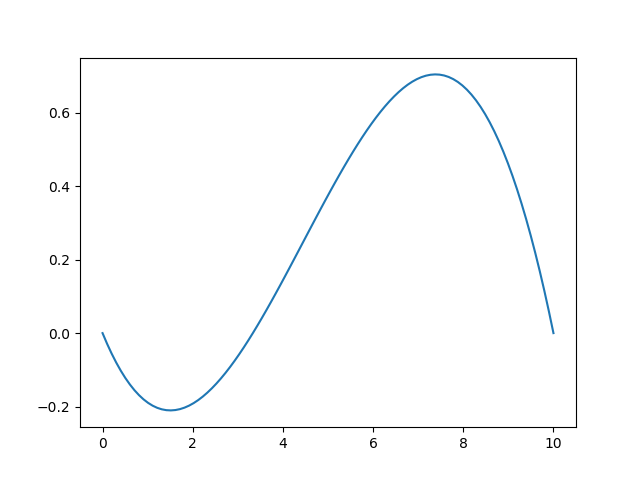
\includegraphics[scale=0.5]{polynominal.png}
        \caption{$\varphi(x)$ for the parameter setting $a=5, b=3, c=0, d=2$}
\end{figure}
Analyzing \eqref{eq:replicator}, this happens if either a strategy
is not present in the population or the excess payoff $\bar{F}(x)$
of a strategy is zero. In the stag hunt game, the fixed points of the
dynamic coincide with the Nash equilibriums of the base game, $f(x) = 0$ for
$x \in \{0,\frac{d-c}{a-b+d-c},1\}$. In general, 
the replicator dynamic lacks the \textit{Nash stationarity} property
and hence there are games with fixed points which are not
Nash\footnote{For a trivial example, consider the prisoners dilemma in 
\ref{prisoners}. A population only consisting of cooperating agents stays in
that state, which is not a Nash equilibrium.} 
\parencite{sandholm_population_2010}.
Concerning fixed points, one is usually interested if the fixed points of 
a dynamic system are stable in terms of some disturbance of the system. 
There are different approaches to stability. A quite strict and useful one 
in the stag hunt game is \textit{asymptotic stability}. 
It essentially requires that a system in a specific fixed point returns 
to the fixed point after a perturbation happend.
\begin{mydef}
        A state of a differential equation is called asymptotically stable
        if ....
\end{mydef}\todo{Exact definition}
Hence, the system tends to move back to an asymptotical stable fixed point
once disturbed. 
A useful theorem to check for asymptotical stability is that 
of \cite{hartmanngrobman}. \todo{State the theorem of hartmanngrobman}
Applying this theorem to the replicator dynamic of the stag hunt game, we find
\section{A simple model of project coordination}
In unversity, students are faced with assignments and projects, which are 
often performed in groups with fellow students.
Nowadays, most of them involve some kind of 
software tool to either present the results, analyze the subject or just
manage the process of aggretating knowledge. Usually the choice of the tools
can be simplified to two possibilities.
One can either use proprietary software
which is usually more user-friendly or choose to rely on free software which
gains in effectiveness by the open community discussing and solving problems
accordingly. Therefore, proprietary software has clearly the disadvantage of
being expensive, resulting in cost for a license for the student or the
institution using it. 

\section{Experimental Evidence}
A third approach beside the traditional and the evolutionary treatment of coordination problems is what \cite{camerer} calls 'fundamental empirical'.
Hence, this section surveys the experimental economic literature regarding 
laboratory coordination games to provide evidence how actual people choose
their strategies in such situations and which factors might influence them. 
Precisely, do people, if they are able to coordinate on an equilibrium at all,
play the risk-dominant or the payoff-dominant equilibrium? And how does their
choice change playing the game repeatedly?
Due to the rich experimental literature on human decisions in social dilemmetas, I will concentrate on studies with frameworks similiar to the evolutionary stag hunt trying to compare the evidence with the results of the theoretical approaches outlined in previous sections. 
\textcolor{red}{Since the papers I will discuss use different notation and 
label strategies different I find it useful to translate theirs into the
notation I used throughout this text. On these grounds, I will call the 
strategy used in the payoff-dominant equilibrium of the stag hunt game
\textit{strategy 1} or in analogy to the stag hunt story \textit{hunting stag}.
Consistently, the strategy used in the risk-dominant equilibrium is called
\textit{strategy 2} or \textit{hunting hare}. Moreover, I use the notation
introduced in section \ref{sec:traditional} to formulate relevant definitions.}
The papers of \textcite{van_huyck_tacit_1990} and \textcite{cooper_communication_1992} are 
seen as the first experiments investigating coordination games \parencite{devetag_when_2007}.
In \textcite{van_huyck_tacit_1990}, subjects do not play a stag
hunt, but an order-statistics game. These games differ in that subjects choose
from a broader set of strategies and hence there are more than two equilibria
in the game. Also the games are played in a group and the payoff to all 
players depend on the lowest strategy one of them chose, thus the name 
'weak-link' order statistics game. Nevertheless, the structure is similiar to 
the stag hunt in the way that the equilibria are Pareto-ranked, with one 
'safe' strategy \parencite{devetag_when_2007}. So evidence from this games is likely to 
be transferable to the coordination problem in the stag hunt game. In 
\cite{van_huyck_tacit_1990} subjects play the order-statistics game in groups of 
14-16 for 10 periods. They only received information about their payoff, but 
so they could find out what the lowest choice of one subject in their group was.
Astonishingly, in every experiment the groups converged
to the equilibrium with the lowest payoff. This result were preserved in another 
five periods of this game although the subjects played an alternative payoff
matrix embracing the payoff-efficient equilibrium across all groups. 
Replications of this results have been performed numerously, with varying group
sizes and slightly changed payoff matrices. One may consult \textcite{devetag_when_2007}
for a summary. 
\textcite{cooper_communication_1992} perform a experiment with a standard two-player stag
hunt game\footnote{They call it simple coordination game(SCG)} 
and one augmented by a dominated strategy. They find that 
subjects in randomly matched one-shot games, knowing only about their own
received payoffs, coordination also fails without any preplay communication. 
However, they find that two-way communication, in which both players were
able to send a message to their matched partner containing which strategy
they intend to choose, solves the coordination problem in the SCG. 
This early approaces suggest that coordination failure\footnote{Here in the 
meaning of not being able to coordinate on the payoff-dominant equilibrium} is
common in laboratory \parencite{devetag_when_2007}. It is noteworthy that the studies 
discussed used different matching protocols, fixed matching in groups and 
random matching against one other player, and yet found the same results. 
A 'very likely consequence of this' is the focus on characteristics of the
payoff matrix in stag hunt games' rather than the implementational details' 
such as the matching protocol \parencite{devetag_when_2007}.

The implementation of random matching in a group is the closest to the 
evolutionary setting discussed in section \ref{evolutionarysection}. This 
procedure was conducted by \textcite{battalio_optimization_2001}. Subjects 
played three stag hunt games with the typical symmetric pure strategy
equilbrium and the symmetric mixed strategy equilibrium at $(0.8,0.2) \in
\Delta$. Figure \ref{fig:payoffbattalio} show the payoff matrices of the
games $2R, R$ and $0.6R$ used. The names become clear when observing the 
\textit{optimization premium} of the games. While controlling for the basin of 
attraction of the equilibria, i.e. the mixed equilibrium is equal across all games,
they want to explore the effect of an increase in the "premium for playing
a best-response" \parencite[751]{battalio_optimization_2001}. 
Therefore they define the optimization premium $r(y)$ of a game $j$ as the 
differece in payoffs choosing the pure strategies $e_1$ and $e_2$ 
while expecting the opponent to play a strategy $y=(q,1-q) \in \Delta$:
\begin{align}
        r_j(y)= \hat{F_j}(e_1,y) - \hat{F_j}(e_2,y) = \delta_j(q-q^*),
\end{align}
with the \textit{optimization premium parameter} $\delta_j$. In the notation
parametrized stag hunt game $\delta_j = a - c + d - b$.
The parameters for the payoff matrices are reported in figure \ref{fig:payoffbattalio}. 
First of all, they find support for their hyptohesis that in games with a 
larger optimization premium subjects coordinated less frequently on the 
payoff-dominant equilibrium. 
Contrary to game $0.6R$, where only one cohort coordinated on the risk-
dominant, in $2R$ no cohort and in $R$ only one cohort converged to the 
payoff-dominant equilibrium. The replicator dynamic does not offer a
a description of this behavior, since convergence to a equilibrium only 
depends on its basin of attractions, which do not differ for the three games, 
and the initial conditions. Whereas "all 24 cohorts start in the basin of attraction
of the risk-dominant equilibrium" \parencite{battalio_optimization_2001}, 
all should converge to the risk-dominant equilibrium according to the dynamic.
In the most cases this is true, with only three exception in game $0.6R$ 
and two in $R$.
But, for the sake of completness, a crossing of the  
"best-response separatrix" \parencite{battalio_optimization_2001} i.e. 
mixed-strategy equilibrium, can not happen in the deterministic replicator 
dynamic.
Furthermore, as they conjectured, a larger
optimization premium increases the speed of convergence. Hence, a coordination
on a equilibrium was achieved fastest in the $2R$ game. 
This is consistend with a postulated replicator dynamic for this games. 
Starting from \ref{replicator}, one can derive that the dynamics of this games
are the same up to a change in speed, proportional to the ratio of 
optimization premia of the games. In game $R$ the change in the population share
playing strategy one is, thus, half the speed of $2R$ and four thirds of $0.6R$,
$\dot{x}_{R} = 0.5 \dot{x}_{2R} = \frac{4}{3}\dot{x}_R$.
\textcite{schmidt_playing_2003} designed their experiment such that the effect
of differing risk levels could be observed. It is convenient to relabel 
the strategies in the game, because in their treatment the payoff-dominant 
equilibria is in the right corner of the normal form game representation,
contrary the notation used throuhout this text. Comparing risk levels between
games, they used a measure due to \cite{Seltenanaxiomaticriskmeasure}, defined
as:
\begin{align}
        \label{riskmeasureschmidt}
        R = ln\left(\frac{\hat{F}(e_2,e_2) -\hat{F}(e_2,e_1)}{\hat{F}(e_1,e_1) 
        -\hat{F}(e_2,e_1)}\right) = ln \left(\frac{d-b}{a-c}\right)
\end{align}
The risk measure $R$ is positive, if the Nash equilibrium $(e_2,e_2)$ is
risk-dominant, and negative if the payoff-dominant equilibrium inhibits both
properties.
None of the four games in \textcite{schmidt_playing_2003} handles
the case of $R=0$, where the mixed-strategy equilibrium is risk-dominant.
In difference to \textcite{battalio_optimization_2001}, they do not
use the proposed optimization premium, but rather measure the risk-dominance 
level in relative terms as $P=\frac{a-d}{a}$.\footnote{As they mention, the 
games in \textcite{battalio_optimization_2001} vary in their level of 
P accordingly.}
The payoff matrices of the games are shown in \ref{fig:payoffschmidt}.
Comparing Game 2 with Game 3, and Game 1 with Game 4, the only difference is the 
degree of risk-dominance and hence one can investigate if subjects react 
to the change in risk-dominance. For game 1 and game 3 the basin of attraction
of both equilibria is equal (Mixed-NE at $(\frac 12, \frac 12)$) and  for
game 2,3 the Mixed-NE is at $(\frac 34,\frac 14)$ resulting in the typical 
larger basin of attraction of the strategy $(e_2,e_2)$. So one would expect
from the replicator dynamic, of course depending on the inital condition 
of the game one, to be more likely attracted to the 'hare-hunting' equilibrium
in game 2,3.
\textcite{schmidt_playing_2003} implement three different types of matching
protocol. First of all, a random matching protocol where each subjects is not
matched twice with another person and only has information about his payoff and
the action of the person he was matched against. 
Secondly, a fixed protocol, matching two persons for several rounds against 
each other, followed by a series of one-shot games. 
In the random matching protcol, they find evidence that an increase in 
risk-dominance, i.e. an increase in $R$, leads to a higher choice of the
strategy in the risk-dominant NE.\todo{Schmidt et al paper.} 

\textcite{dubois_optimization_2012} conduct a similiar experiment as 
\textcite{schmidt_playing_2003} and \textcite{battalio_optimization_2001},
but introduce a different measure for the risk subjects are confronted with in
the games. They define the \textit{relative riskiness} of a games 
"safe strategy relative to the risky strategy" as $RR = \frac{|c-d|}{a-b}$.
Intuitively, a player commited to strategy one and calculating the 
difference a deviation of the other player from strategy one to two, gets
$(a-b)$. Similiary for strategy two, he receives $c-d$. The relative riskiness
measure is, hence, the ratio of those deviation calculations. Alternatively,
it can be interpreted as the ratio of the standard deviations of the payoffs 
\parencite{dubois_optimization_2012}. They speak of "comparable riskiness",
if the $RR$ measure is close to one \cite{dubois_optimization_2012}. 
According to $RR$, the risk-dominant strategy 2 is said to be less risky 
relative to the payoff-dominant strategy 1 in on game compared to another if 
$RR$ is smaller.
Observing the values of the relative riskiness by 
\textcite{dubois_optimization_2012} and the risk-dominance measure of 
\textcite{schmidt_playing_2003} for the games used in the papers, it is clear
that both measures are in a conflict. As by \textcite{schmidt_playing_2003}
measure, risk-dominance is kept constant in the games of 
\textcite{battalio_optimization_2001}, relative riskiness indicates a 
variation. On the other hand, relative riskiness cannot distinguish between
the games 1,2 and 3 of \textcite{schmidt_playing_2003}, since $RR=0$. In an
early working version of their paper they explicitly excluded the case 
$c \neq d$ and statet that "a more general measure of relative riskiness 
should allow for the case where c=d as compared to $(a-b)$ 
\parencite{dubois_optimization_2008_working}. 
\todo{Maybe both measures capture different things: Intuition}
With the implementation of game 1 a replication of the results for 
\textcite{battalio_optimization_2001}'s game $0.6R$ could be 
performed\footnote{The payoff matrices are identical. 
Compare \ref{fig:payoffdubois} and \ref{fig:payoffbattalio}}. 
As per their conjecture they found that a lower relative riskiness in a game 
decreased the rate of choice of strategy one, keeping the optimization premium 
constant. This is congruent with the intuition that the severity of the impact 
related with the strategic uncertainty subjects face in a game, expressed in
the difference in payoff a deviation of the other player would cause,
effects the choice of the strategy. 
On the other hand, keeping the relative riskiness constant and varying the
optimization premium, they cannot find an effect on the frequency of 
strategy 1. 
In measuring the "coordination sucess", they deploy the concept of "strong
coordination". 
In other words, counting the occurence of periods in which a group
uniformly adopts a strategy such that every pair of subjects lands in one
of the Nash equilibria. \textcite{dubois_optimization_2012} intend to sort 
out "furtuitous coordination", coordination as consequence of subjects being
randomly matched with each other. Comparing strong coordinations between the
games they find a non-significant difference between game 1 and game 2 in 
which only the relative riskiness certeris paribus was changed. Contrary to 
that there is a significant difference in the commoness in game 3 to game 2.
Since game 3 and game 2 only differ in their optimization premium 
\textcite{dubois_optimization_2012} conclude that a higher optimization
premium leads to more (strong) coordination. As they mention, this agrees
with the observation of \textcite{battalio_optimization_2001} that the 
speed of convergence hinge positively on the optimization premium. \todo{
Is it really the convergence or did I miss something?}
\todo{History of Play}

As seen from the evidence \textcite{battalio_optimization_2001},
\textcite{schmidt_playing_2003} and \textcite{dubois_optimization_2012} 
found, the structure of the payoff matrix has a strong impact on the way 
people play the stag hunt game.   
The story this evidence tells is quite frightening. Failure to coordinate 
on the payoff-dominant equilibrium seems to be common. Following an argument
of \textcite{kreps_game_1990} that identical strategic interactions, such
as the play of completely indentical stag hunt games in the laboratory,
"take us very little distance outside the laboratory", 
\textcite{rankin_strategic_2000} design an experiment with a randomly 
pertubated stag hunt game. Essentially, the payoff to strategy 1 is fixed 
whereas the payoff to strategy 2 varies randomly between the games. This is
depicted in the payoff matrix \eqref{eq:payoffrankin}.
\begin{align}
        \label{eq:payoffrankin}
        A = \mqty(1 & 0 \\ x & x)
\end{align}        
The parameter $x$ is equally distributed between $(0,1)$ and once a sequence
was calculated used for all cohorts participating in the experiment. This
variation justifies to describe the games as "similiar" but not
"identical", hence the structure stays the same, but the risk-dominance 
property varies. Indeed, if $x$ is greater than $0.5$ risk-dominance and
payoff-dominance select different equilibria, $(e_2,e_2)$ and $(e_1,e_1)$,
respectively. For a value of $x$ smaller than $0.5$ both select the 
the equilibrium in strategy 1. One finds that the optimization premium for 
this randomly perturbed games does not change, since $\delta=1-x+x+0=1$. 
The relative riskiness measure $RR$ cannot discriminate between this games,
since $|d-c|=0\ \forall x$. \cite{schmidt_playing_2003} measure of risk of 
course is positive for $x > 0.5$ and negative for $x <0.5$
The question \textcite{rankin_strategic_2000}
want to investigate is, if this framework of sligthly varied situations may
lead the groups to form a "convention" which deductive principle to choose. 
In contrast to the studies performed with identical stag hunt games, they 
observe emerging coordination to the payoff dominant equilibrium across
all cohorts. Whereas in the first ten periods of play risk dominance seems
to have some explanatory power for the choice of strategy, in the last ten
rounds 91\% choose the payoff dominant action. 
In the cases of coinciding equilibrium selection of risk-dominance and payoff-
dominance ($x < 0.5$) all subjects coordinated on that equilibrium in group
1-5 and 95\% of the subjects in group 6. But also for the other case a high
coordination on the payoff-dominant strategy was observed, ranging from 
80\% to 95\% of the strategies played, suggesting that there is clear evidence
for the hypothesis of an emerging convention based on the deductive principle
payoff-dominance. This sends a quite positive image about coordination, because 
this is "dramatically at odds with claims that coordination failure is common"
\parencite[9]{devetag_when_2007}. 
As outlined, the most studies concerned with the stag hunt game in the 
laboratory focused on the payoff matrix. However, implementational details 
such as the matching protocol influence behaviour sharply. Not only 
\textcite{van_huyck_tacit_1990} found in their two-player fixed matching
convergence to the payoff-dominant equilibrium, 
\textcite{clark_repetition_2001} also found different strategy 
choices between randomly matched one-shot games and fixed matching protocol 
games. The latter lead to significantly higher choices of the strategy 
in the efficient equilibrium and less "disequilibrium play" in general. 
\textcite{devetag_when_2007} mention that this one-shot games imply a 
random matching protocol. But it is different to random matching on group
basis, where subjects can play against the same opponent again 
and hence there is the possibility that a "convention" emerges like in 
\cite{rankin_strategic_2000}.

Even more subtle experiment design differences are conjectured to have an
effect. For example \textcite{devetag_when_2007} suggest that the formulation
"you will remain grouped with the same seven other participants for the next
75 rounds" in the instruction of the \textcite{rankin_strategic_2000} 
experiment may increased trust within the group and hence was a 
cause for the exceptional coordination success. Comparatively, the 
instructions in \textcite{dubois_optimization_2012} read "At the beginning
of each period, in each group (composed of 8 participants), the computer
system will form 4 pairs of subjects. [...] The experiment 
involves 75 rounds". While essentially containing the same information,
it does not emphasize the fact that subjects can reencounter the same 
players again. 

An interesting experimental approach is executed by 
\cite{dufwenberg_gender_2005}. They try to evaluate if there is a diffrence
in coordination behaviour accross genders, motivated by the different
treatment of males and femals in the work place. Playing the weak-link order
statistics game in \cite{van_huyck_tacit_1990}, groups of only femals or only
males face the coordination problem with Pareto-ranked equilibria. The 
motivation of observing gender differences was "never explicitly pointed 
out to the subjects" \parencite{dufwenberg_gender_2005}\footnote{
Even though it might be interesting to see if there is an effect like 
the discussed "crab basket" effect which leads woman to mistrust each other 
more than in a mixed group.} However, they do not find that the groups play
different. Differences in the beginning "disappear fast" and "no difference
is found in later stages". All groups converge to the choice of the minimum
contribution. As they mention, it might be useful to investigate differences
with groups that also have some other characteristica in common. They refer
to the differences group identity has for femals and males playing a 
public goods game. Namely \textcite{croson_groups_2008} found that when
females in a sorrority play the public goods games they perform better than 
females with no specific belongingness. Contrarly, males in a fraternity 
performed worse than males without a group identity. 
Interestingly, this and other factors concerning the group of subjects 
playing the coordination game might be a rationale for the initial conditions
in the evolutionary dynamic. The intitial conditions might be used to 
capture the composition of the subjects interacting in reflecting how well
trust or some kind of cultural risk aversion is embedded as convention. 
Nevertheless, it seems difficult, atleast for the author, to justify
the reduction of culture to one\footnote{Of course, in games with more 
than two strategies the initial conditions are represented by a vector}
dimension such as $x_0$
\todo{External validity}

The discussion of the laboratory research makes on clear: There is more
to the coordination problem than individuals programmed like a robot 
to a strategy, while being attracted and moved to an equilibrium by a dynamic
in a fully deterministic fashion. But, as a model should, the analysis offers 
a simplification that helps to understand some of the patterns observeable 
when real people interact.
\section{Application and Outlook}
\section{appendix}
\begin{figure}[h]
        \label{fig:payoffbattalio}
\caption{Payoff matrices of games in \textcite{battalio_optimization_2001}}
\begin{alignat*}{3}
        A_{2R} &= \mqty(45 & 0 \\ 35 & 40) \quad & &A_{R} = \mqty(45 & 0 \\ 
        40 & 20) \quad & &A_{0.6R} = \mqty( 45 & 0 \\ 42 & 12) \\
        \delta_{2R} &= 50  \quad & &\ \delta_{R} = 25 \quad & &\ \delta_{0.6R} = 15
\end{alignat*}
\end{figure}
\begin{figure}[H]
\label{fig:payoffschmidt}
\caption{Payoff matrices of the games used in \cite{schmidt_playing_2003}}
\begin{alignat*}{3}
        A_{Game1} = \mqty( 100 & 20 \\ 60 & 60), \quad A_{Game2} 
                               &= \mqty( 100 & 20 \\ 80 & 80), \\ 
        A_{Game3} = \mqty( 100 
             & 60 \\ 80 & 80), \quad A_{Game4} &= \mqty( 100
                             & 0 \\ 80 & 60)
        \end{alignat*}
\end{figure}
\begin{figure}[H]
        \caption{Payoff matrices of the games used
        in \cite{dubois_optimization_2012}}
        \label{fig:payoffdubois}
        \begin{alignat*}{3}     
                A_{Game1} &= \mqty(45 & 0 \\ 42 & 12),
                A_{Game2} &= \mqty(40 & 20 \\37 & 32),
                A_{Game3} &= \mqty(44 & 4 \\ 38 & 28) \\
                RR_{Game1}&= \frac 23, RR_{Game2}&=\frac 14, RR_{Game3}&=
                \frac 14
        \end{alignat*}
\end{figure}
\printbibliography
\end{document}







